% Chapter X

\chapter{Simulating Collisions in Thermal Gases} % Chapter title

\label{ch:inhomogas} % For referencing the chapter elsewhere, use \autoref{ch:inhomogas} 

%----------------------------------------------------------------------------------------

\begin{flushright}{\slshape    
When I write, I feel like an armless,\\
legless man with a crayon in his mouth.} \\ \medskip
--- Kurt Vonnegut
\end{flushright}

\bigskip

%----------------------------------------------------------------------------------------

Introduce section motivate use for the classical method (ease of simulation outside of equilibrium, no need to assume ergodic motion etc), flow to DSMC method.

%----------------------------------------------------------------------------------------

\section{The DSMC Method} \label{sec:dsmc}

Originally developed by Bird for dilute gas flow in engineering and space science \cite{Bird1963,Bird1976,Bird1994}, the Direct Simulation Monte Carlo (DSMC) method has become a well-established technique for the numerical simulation of gas flows at the molecular level \cite{Bird2013}.
Since its inception, the DSMC method has been successfully utilised in a diverse range of physics: from problems in microelectromechanics systems (MEMS) \cite{Frangi2003} to Volcanic plumes on Jupiter \cite{Zhang2004}, from solutions to fundamental flows like Rayleigh-B\'enard flow \cite{Watanabe1994} to investigating the complex dynamics of chemically reactive flows \cite{Anderson2003,Goldsworthy2014}.
More specifically (?) the DSMC method has enjoyed continuued success in the field of cold atom physics: with evaporative cooling and expansion dynamics \cite{Wu1996, Wu1997, Wu1998}, bosonic collective mode dynamics \cite{Jackson2001, Jackson2001b, Jackson2002, Jackson2002b, Jackson2002c}, fermion dynamics \cite{Urban2006, Urban2007, Urban2008, Lepers2010} (see also \cite{Vignolo2002, Toschi2003, Capuzzi2004, Toschi2004}), sympathetic cooling \cite{Barletta2010, Barletta2011} (REWORD) and high-energy collisions of thermal clouds \cite{Wade2011}.

\marginpar{The Knudsen number is the ratio of the mean-free path to the representative length scale of the system. It is useful for determining the scale of the fluid flow. If the Knudsen number is near or greater than one, the mean free path of a particle is comparable to a length scale of the problem, and the continuum assumption of fluid mechanics is no longer a good approximation.}
The unifying attribute for the above examples is that they are all dilute gases, that is each flow will typically have a \emph{Knudsen number}, $Kn$, greater than one.
As we saw in \autoref{sec:mfp}, standard cold atom experiments are in the collisionless regime ($Kn>1$), although as the density of the gas increases with evaporative cooling the Knudsen number reduces.
\textcolor{blue}{I want to make a comment on the increase in computational intensity as the Knudsen number reduces here, but I am unsure how to do it. ** Exact quote from Goldsworthy ** The dependence of computational expense with the level of rarefaction occurs because potential simulator particle collision pairs must be separated by a distance less than the local mean free path, and so the smaller $l$, the greater the number of simulator particles required. }

%Compare to molecular dynamic approaches, when is DSMC appropriate / good? When does it fail? 
The obvious way to tackle simulating particulate gases might be to employ a deterministic molecular dynamics (MD) \cite{Alder1957} type approach.
While MD techniques have been accurately simulating molecular fluid flows for over 6 decades \cite{?,?,?} they are better suited to dense gases.
The drawback with the MD method is that for a given physical problem the number of simulated particles is not a free parameter.
Bird uses the example of the number of molecules, $N_l$, contained within a cube with side length equal to one mean free path length, $l$.
For a typical\footnote{For this calculation I considered an atomic gas in a quadrupole trap with $B_z=2.5\,\mathrm{Tm}^{-1}$, from a temperature of $200\,\mu\mathrm{K}$ with $10^7$ atoms to a temperature of $20\,\mu\mathrm{K}$ with $10^6$ atoms.} cold atom experiment this number might range from $10^{14}$---$10^{18}$.
Clearly this number of particles is intractable computationally, as we would require something on the order of $5$---$500\,\mathrm{PB}$ to store the position and velocity of each particle.

%Describe DSMC method.
\marginpar{In a typical implementation of the DSMC method it is sufficient to have $\alpha > 1$, where each simulator particle is a \emph{superparticle} representative of a number of physical atoms. In this instance $\alpha$ is simply a numerical tool to increase computational efficiency. However in simulations of highly non-equilibrium dynamics it can be essential for $\alpha \ll 1$ to ensure accurate results \cite{Wade2011}.}
The DSMC method uses a cluster of simulator particles to represent the distribution function of the Boltzmann equation,
\begin{equation*}
    f(\mathbf{p},\mathbf{r},t) \approx \alpha h^3 \sum_{i=1}^{N_s}\delta\left[\mathbf{p}-\mathbf{p}_i(t)\right]\delta\left[\mathbf{r}-\mathbf{r}_i(t)\right],
\end{equation*}
where $\alpha = N_p / N_s$ is the ratio of physical atoms, $N_p$, to simulator particles\footnote{Throughout this text I will distinguish between real physical atoms (or molecules) and numerical simulated atoms with the designations atom and particle respectively.}, $N_s$.
The crucial assumption of the DSMC method is that this distribution function can be used to approximate a solution to the Boltzmann equation by decoupling the deterministic dynamics of the atomic motion from the statistical inter-particle interactions.
Thus the algorithm can be considered in two sections: the Newtonian evolution of the particle cluster, and the probabilistic collision energy exchange.

The specific implementation of the integration of particle motion is left up to the programmer to decide, since different problems will require differing levels of accuracy and efficiency.
However it is strongly advised that the integration method be symplectic to ensure conservation of energy, in my simulations I have implemented a version of the velocity Verlet method \cite{verlet1967}, a fourth order, ${\cal O}(\Delta t^4)$, in position and second order, ${\cal O}(\Delta t^2)$, in velocity, symplectic integrator that is the linchpin of many MD simulations. 

The way in which the DSMC method handles collisions is the source of the methods true brilliance.
Collisions are simulated probabilistically in small regions of space called cells.
These cells are implemented as an efficient means to find nearest neighbour collision pairs.
\marginpar{The technique employed by the DSMC method for selecting collision pairs reduces the overall computational cost from ${\cal O}({N_s}^2)$ to ${\cal O}(N_s)$.}
The number of pairs chosen and the probability with which they collide is then optimised to reduce the number of null pairs.
In my simulations I have implemented the specific algorithm developed by Wade et al \cite{Wade2011} whereby
\begin{equation}
    P_{ij} = \alpha \frac{\Delta t}{\Delta V_c} v_r \sigma(v_r),
\end{equation}

\begin{subequations}
\begin{align}
    &P_{ij} \to \tilde{P}_{ij} = \frac{P_{ij}}{\Lambda},\\
    &M_{c}  \to \tilde{M}_{c}  = M_{c} \Lambda,
\end{align}
\end{subequations}

\begin{equation}
    \Lambda = \frac{ \ceil*{M_c \alpha \frac{\Delta t}{\Delta V_c} \left[ v_r\sigma(v_r) \right]_\mathrm{max} } }{M_c},
\end{equation}
\begin{equation}
    \tilde{M}_c = \ceil*{ \frac{N_c-1}{2}n_c\Delta t \left[v_r\sigma(v_r)\right]_{\mathrm{max}} },
\end{equation}
where
\begin{equation}
    n_c = \alpha N_c / \Delta V_c,
\end{equation}
is the density of the cell.


Refer to cuda \autoref{ch:cudadsmc} Should also discuss the development of this parallel implementation of the code. Compare to CPU implementations. Goldsworthy \cite{Goldsworthy2014} has a few references for other CUDA codes.

%----------------------------------------------------------------------------------------

\section{DSMC simulations of collisions}

The heart of the DSMC method is to simplify the simulation of interparticle interactions in the form of two body collisions.
In this sense there are two aspects we need to ensure are modelled accurately; the number and frequency of collisions (collision rate) and the collisions themselves, wether or not they are correctly distributing the kinetic energy.
In the following sections I carefully analyse these two aspects to ensure the utmost accuracy in our simulations.

The DSMC method offers some free parameters which we can optimise to balance the accuracy and efficiency of the algorithm, namely the number of cells, $n_c$, and the number of test particles, $N_p$.
We wish to see the effect of varying these parameters on the results of the simulation.

**Include a surface plot of the collision rate as a function of cell number and test particle number.
Should make the z axis percentage error. See fig 14. in wade. **

\begin{figure}
\hspace{-8em}
\makebox[1.8\linewidth][l]{%
\centering
\subfloat[Homo err]{\label{fig:a}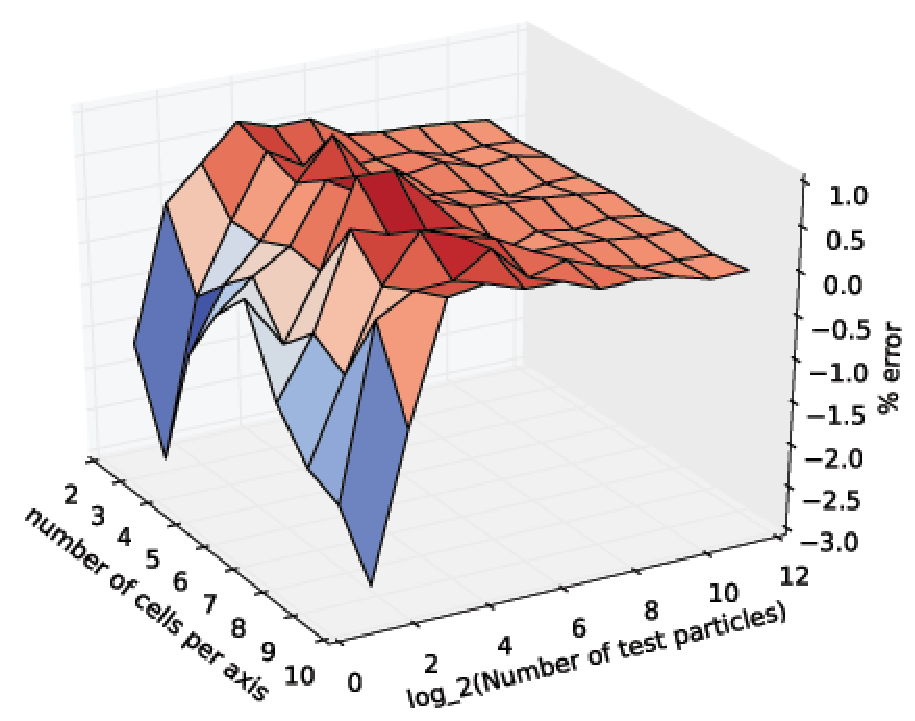
\includegraphics[width=0.525\textwidth]{gfx/HomoError}}%
\subfloat[IP err]{\label{fig:b}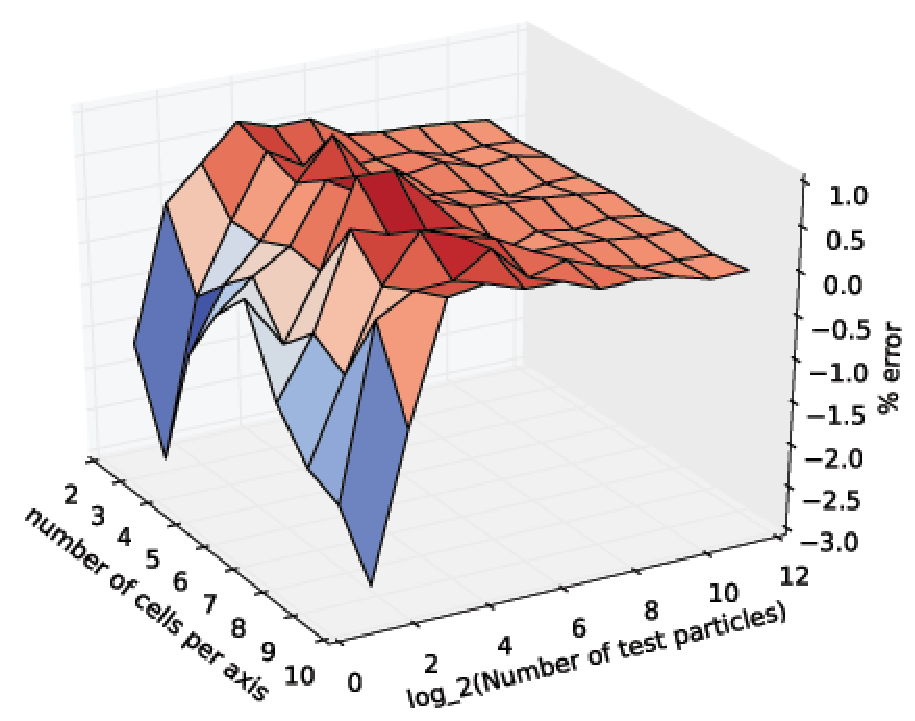
\includegraphics[width=0.525\textwidth]{gfx/HomoError}}%
\subfloat[Quad err]{\label{fig:c}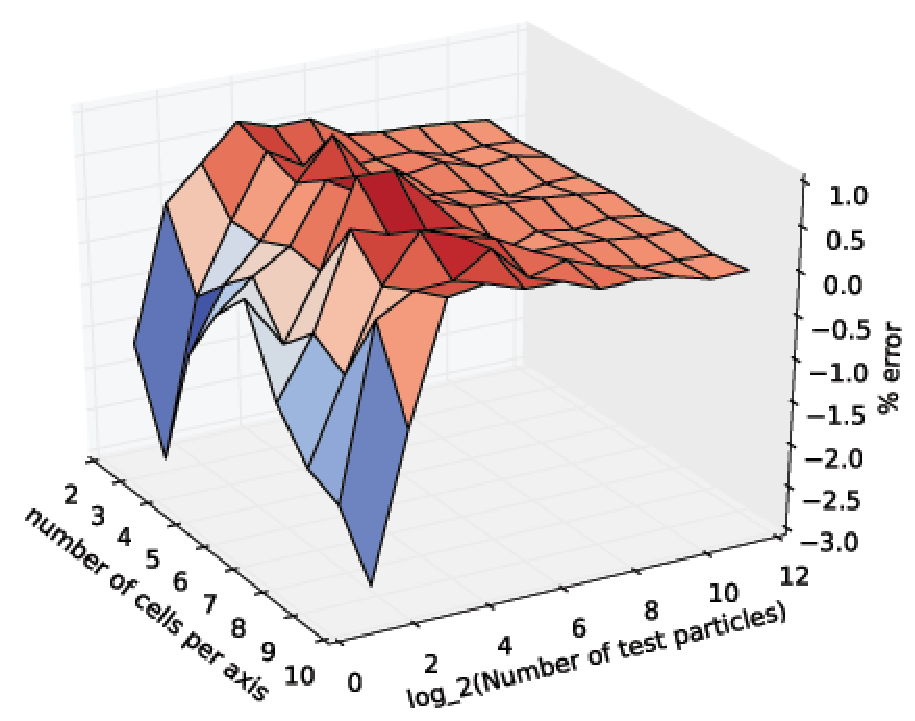
\includegraphics[width=0.525\textwidth]{gfx/HomoError}}%
}
\caption{Error of DSMC method as a function of test particle number and cell number.}\label{fig:dsmccolerr}
\end{figure}

Figure \ref{fig:dsmchomoerr} shows how well the DSMC method performs over a wide range of test particle and cell numbers in a homogeneous gas. 
We can see in the corner the method beginning to fail. 
This is the region where, on average, we have less than two test particles per cell. 
This means that there is not enough atoms to perform a collision within a cell. 
One way to avoid this (which has not been implemented here) is to search neighbouring cells for collision pairs when a partner can not be found in the current cell.
The main thing to observe here is the increase in the error as the number of test particles is reduced.

Smaller cells -> larger fluctuations.

Not adaptive since slowly changing cloud.


%----------------------------------------------------------------------------------------

\section{Thermalisation} 

Now that we are convinced an atomic gas, simulated with the DSMC method, has a physically correct collision rate, we must confirm that collisions distribute energy as we expect.
\marginpar{Thermalisation is the generic name for all kinds of processes giving rise to relaxation towards thermal equilibrium starting from a non-equilibrium situation \cite{Walraven2010}.} 
The perfect way to test this is through an investigation of \emph{thermal relaxation} or the process of thermalisation through elastic collisions.
There are many ways that a system can be out of thermal equilibrium, but here I will consider two scenarios that have generally accepted solutions to which we can compare our simulations.

\subsection{Thermal Relaxation after a Thermal Perturbation} \label{sec:walravenTherm}

The simplest example for rethermalisation\footnote{A more common terminology for thermal relaxation is rethermalisaiton \ie\,to return to the thermal distribution.} is somewhat reminiscent of evaporative cooling, that is the case of simply perturbing equilibrium by adding a small number of atoms whose average energy is different to that of the bulk gas\footnote{Obviously evaporative cooling is simply the removal of atoms whose total energy is different from the average of the bulk.}.
In \cite{Walraven2010} Walraven shows that the rethermalisation time\footnote{That is the $1/e$ time.}, $\tau_\mathrm{th}$, is given by
\begin{equation}
    \tau_\mathrm{th} = 2\left(\gamma + 3/2\right)\tau_{c}. \label{eq:walravenRetherm}
\end{equation}
Using the values for the trapping parameter, $\gamma$, given in \autoref{tab:collisionrates} we find the rethermalisation time in a homogeneous, IP and quadrupole trap to be 3, 6 and 9 times the collision time in each trap respectively.

Anderlini and Gu\'ery-Odelin \cite{Anderlini2006} have taken this analysis one step further, considering the effect of including all partial waves in the collision integrals has on a homogeneous box trap and a harmonic potential.
Interestingly in the limit of constant cross section the results for the homogeneous trap reduces to that given in \autoref{eq:walravenRetherm} with $\gamma=0$, ($\tau_\mathrm{th}=3\tau_\mathrm{c}$).
In fact they go on to show that for the harmonic trap the rethermalisation time is longer by a factor of 2, which again, agrees with \autoref{eq:walravenRetherm} for $\gamma=3/2$, ($\tau_\mathrm{th}=6\tau_\mathrm{c}$).

Before we tackle this scenario numerically the reader might be a little confused by the above result. 
Looking at equation \autoref{eq:walravenRetherm} it is quite clear that as the trapping parameter, $\gamma$, increases the number of collision required for rethermalisation increases.
Aderlini et al. explain this best when they say
\begin{displayquote}
    \dots the fact that the space of configuration is larger for a nonhomogeneous gas, and that the thermalization affects both the space and velocity degrees of freedom.
\end{displayquote}
We can understand this statement better if we consider an effective volume in configuration space, $V_\mathrm{cs}$, (analogous to the effective volume in real space, $V_{e}$)
\begin{equation}
    V_\mathrm{cs} = \int \exp\left[ -\frac{H( \mathbf{r}, \mathbf{v})}{k_B T}\right]\,d\mathbf{r}d\mathbf{v} = V_e \left(\frac{3\pi m}{k_B T}\right)^{3/2}.
\end{equation}
So we can see that for a given temperature the region occupied in configuration space increases with the effective volume, which \autoref{tab:collisionrates} shows increases with $\gamma$.
Again this might make the reader uncomfortable, we seem to have convincingly shown that tighter trapping potentials take longer to rethermalise. 
We stated in \autoref{sec:collisionRates} that evaporative cooling, a process driven by thermal relaxation is more efficient in tighter trapping potentials \ie\,larger trapping parameters.
So how can this be?
As I will show in \autoref{sec:evaporation}, even though these traps take longer to rethermalise they have greater gains in density for a given number of lost atoms during evaporation.

\begin{figure}
\hspace{-8em}
\makebox[1.8\linewidth][l]{%
\centering
\subfloat[Walraven homegeneous gas thermalisation. $\tau_{c}^{-1} / \tau^{-1} = 1.2$ should equal 3?]{\label{fig:walravenHomo}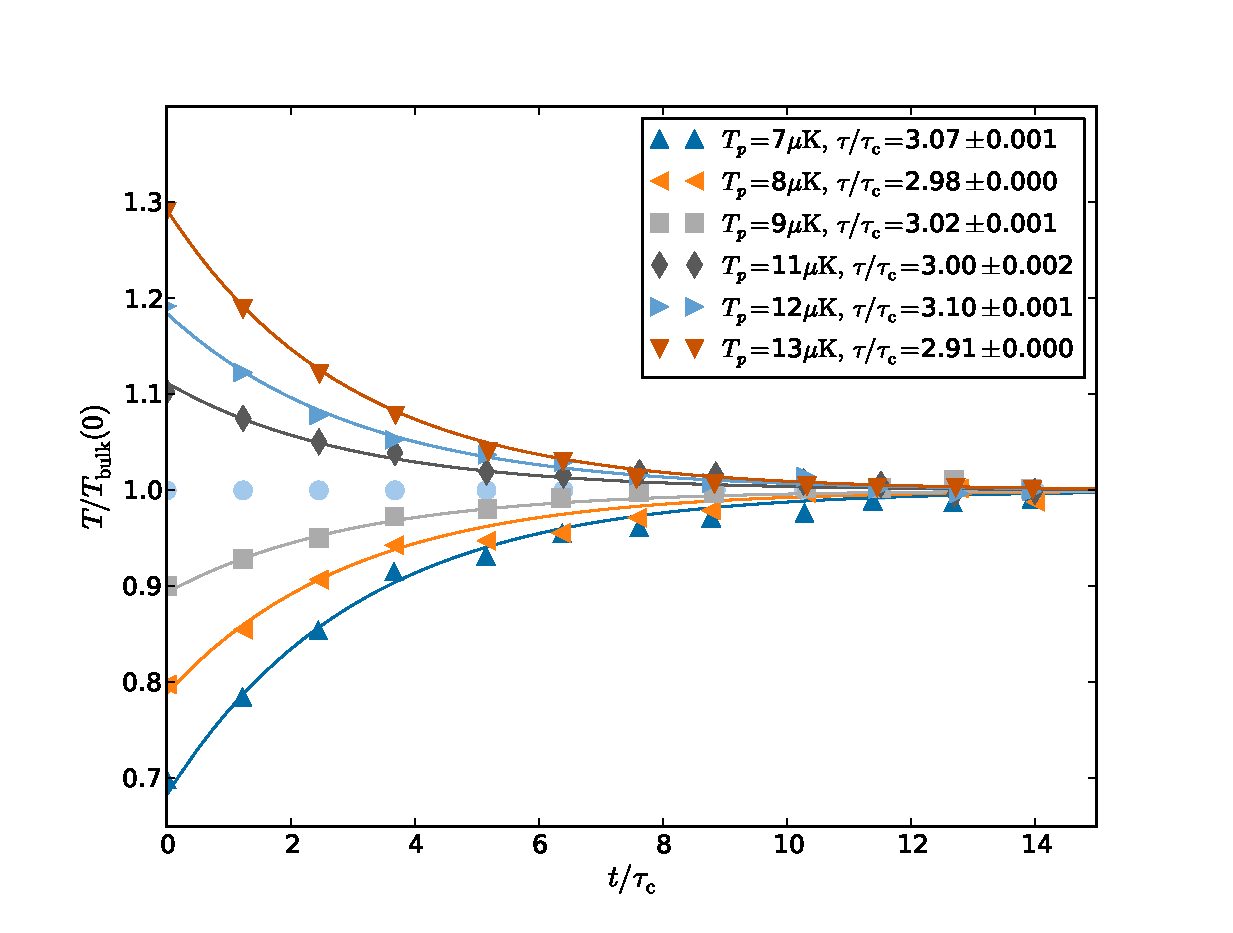
\includegraphics[width=0.525\textwidth]{gfx/Thermalisation/walravenHomo}}\quad
\subfloat[Walraven ip gas thermalisation. $\tau_{c}^{-1} / \tau^{-1} = 1.6$ should equal 6?]{\label{fig:walravenIP}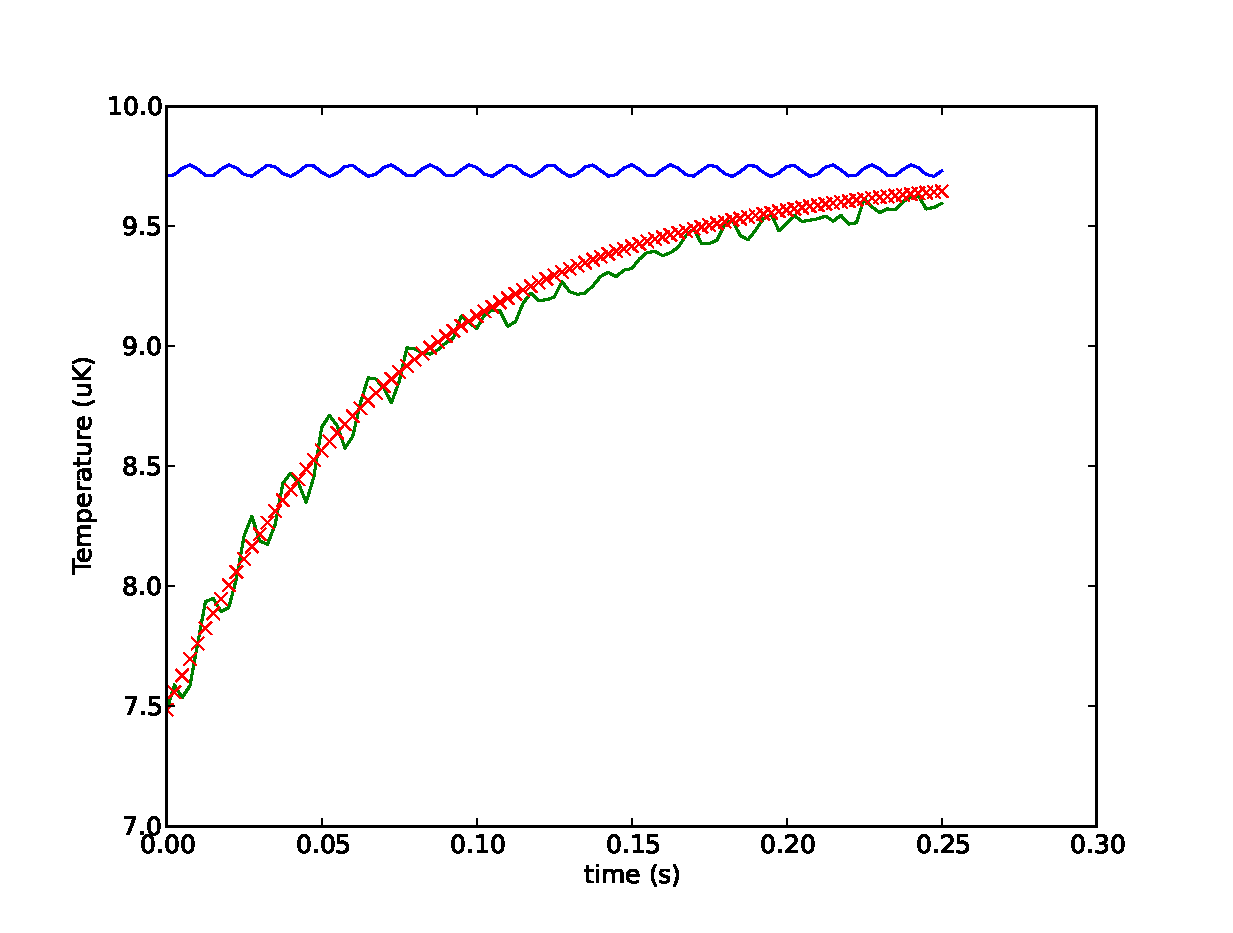
\includegraphics[width=0.525\textwidth]{gfx/Thermalisation/walravenIP}}\quad
\subfloat[Walraven quad gas thermalisation. $\tau_{c}^{-1} / \tau^{-1} = 10.45$ should equal 9?]{\label{fig:walravenQ}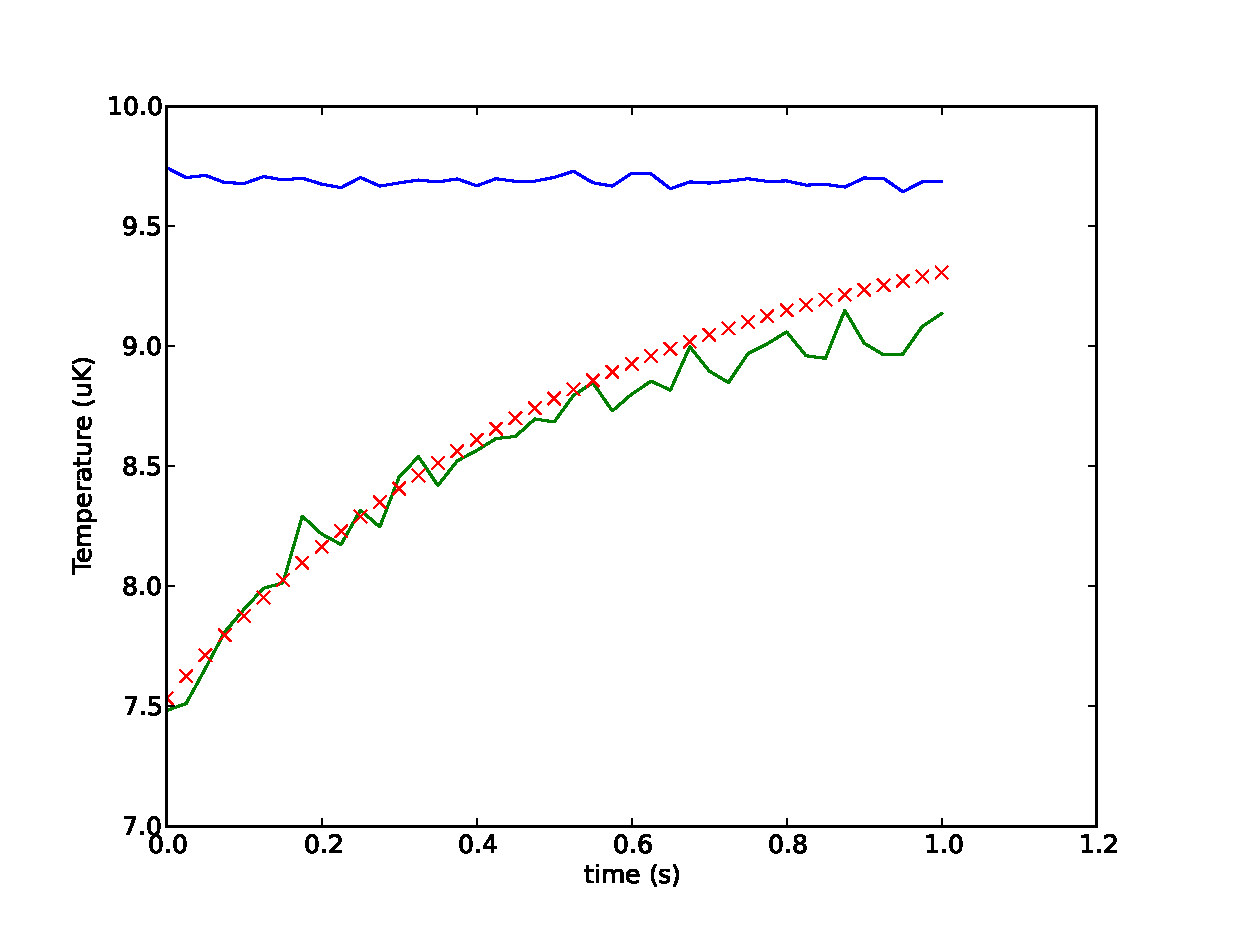
\includegraphics[width=0.525\textwidth]{gfx/Thermalisation/walravenQuad}}%
}
\caption{Walraven rethermalisation. I want to do this simulation for some different perturbation temperatures. One more higher and one lower too.}\label{fig:walravenTherm}
\end{figure}

In \autoref{fig:walravenTherm} we have simulated a million physical atoms, $N_P=10^6$, at $10\,\mu \mathrm{K}$ in three different trapping potentials: homogeneous, IP and quadrupole. 
Each gas began in an initially thermal distribution with 1\% of the particles at set to have an average temperature of $7,8,9,11,12,13\,\mu\mathrm{K}$.
\marginpar{When choosing the initial perturbed distribution we must keep in mind the virial theorem \cite{}. The key result here is that in a thermal distribution we have $\langle E_p \rangle = \frac{2\gamma}{3} \langle E_k \rangle = \gamma k_B T$. So when choosing the width for the spatial distribution we must keep in mind the effective power of the trapping potential. }
For each simulation we have chosen the trapping parameters such that the collision rate was approximately 25 collisions per atom per second, as this number is similar to atoms of this temperature in an evaporation experiment.
We used one million test particle, $N_T=10^6$, in each simulation so that the ratio of physical atoms to test particles was one, $\alpha=1$.

For the homogeneous gas simulation shown in \autoref{fig:walravenHomo} I set the width of the box containing the atoms to be $100\,\mu \mathrm{m}$ in each direction. 
This corresponds to a collision rate of $24.64\,\mathrm{s}^{-1}$.
I found the thermalisation occurred in $3.14\pm 0.02$ collision times, closely resembling the result in \autoref{eq:walravenRetherm}.

For the Ioffe Pritchard trap simulation shown in \autoref{fig:walravenIP} we set $B_0=0.01\,\mathrm{T}$, $B'=33.54\,\mathrm{Tm}^{-1}$ and $B''=75,000\,\mathrm{Tm}^{-2}$ which equates to a ${B_{\rho}}''=75,000\,\mathrm{Tm}^{-2}$. 
Choosing these trapping parameters gives a collision rate of $24.72\,\mathrm{s}$.
I found the thermalisation occurred in $6\pm 0.1$ collision times, again, in perfect agreement with \autoref{eq:walravenRetherm}.

Finally in the quadrupole trap simulation shown in \autoref{fig:walravenQ} we set $B_z=2.8\,\mathrm{Tm}^{-1}$ resulting in a collision rate of $25.48\,\mathrm{s}$.
I found the thermalisation occurred in $9\pm 0.1$ collision times, again, in perfect agreement with \autoref{eq:walravenRetherm}.

We can note from all simulations shown in \autoref{fig:walravenTherm} that the thermalisation time appears to be independent of the size of the perturbation. 
Not truue large perturbations tend to thermalise i different times.

Also talk about cell number, correct resolution and not thermalising in the correct time.

\subsection{Monroe Thermalisation}

Another interesting experiment that has been investigated in some depth is the rethermalisation of a directional anisotropy. 
In these experiments the kinetic energy is changed in one cartesian direction only (the spatial distribution is reshaped accordingly), creating a directional anisotropy in the distribution.
This squeezed distribution is then allowed to rethermalise through elastic collisions.
The original theoretical development of Myatt \cite{Myatt1997} predicts that in a harmonic trap the thermalisation time for a directional anisotropy is approximately 2.7.
This result has been used to experimentally determine the collision cross section, $\sigma$, of atoms in ultra-cold gas experiments \cite{Monroe1993, Davis1995}. 

Snoke and Wolfe \cite{Snoke1989} also considered the rethermalisation of homogeneous gas with a non-thermal initial distribution.
They found that no matter what the initial distribution their simulated gases always tended to a Maxwell-Boltzmann distribution in less than 5 collisions.

Wu and Foot \cite{Wu1996} have repeated these simulations (both those of Myatt and Snoke and Wolfe) using the DSMC method.
Their simulations agreed with the predictions of Myatt for the case of the harmonic trap, while they found that directional anisotropies in a homogeneous gas thermalised in fewer collisions than in a trapped gas (as we might expect given the result in \autoref{eq:walravenRetherm}).

Here I have extended this investigation to consider the rethermalisation times in our three favourite trapping potentials: homogeneous, Ioffe Pritchard and quadrupole.
As we saw in \autoref{sec:walravenTherm} we can't expect the thermalisation time to be the same in different trapping potentials.
In fact, when the perturbation was kept constant, the thermalisation time was purely a function of the trapping parameter, $\gamma$.

\begin{figure}
\hspace{-12em}
\makebox[1.8\linewidth][l]{%
\centering
\subfloat[Monroe homegeneous gas thermalisation. $\tau_{c}^{-1} / \tau^{-1} = 0.77$]{\label{fig:monroeHomo}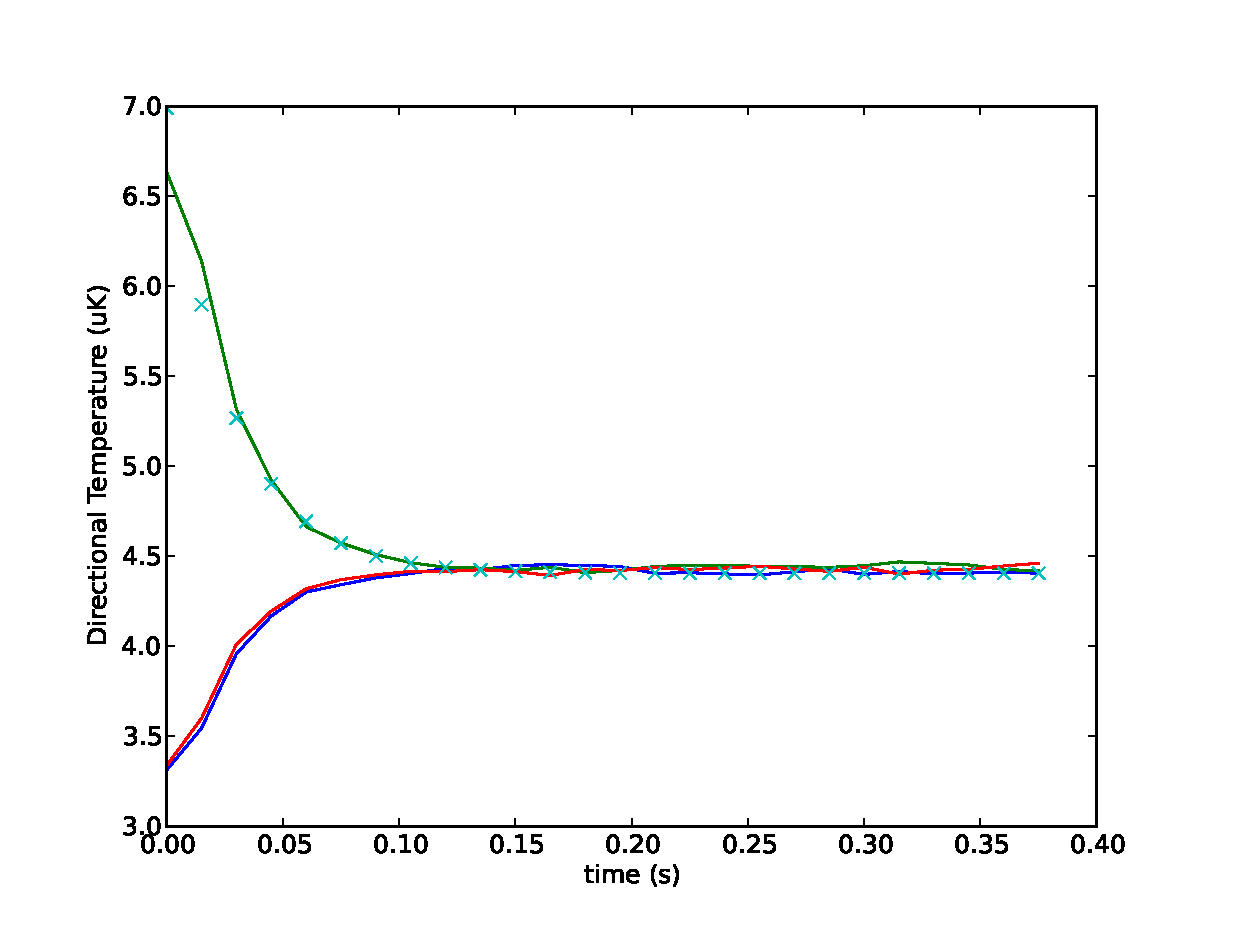
\includegraphics[width=0.525\textwidth]{gfx/Thermalisation/monroeHomo}}\quad
\subfloat[Walraven homegeneous gas thermalisation. $\tau_{c}^{-1} / \tau^{-1} = 2.21$]{\label{fig:monroeIP}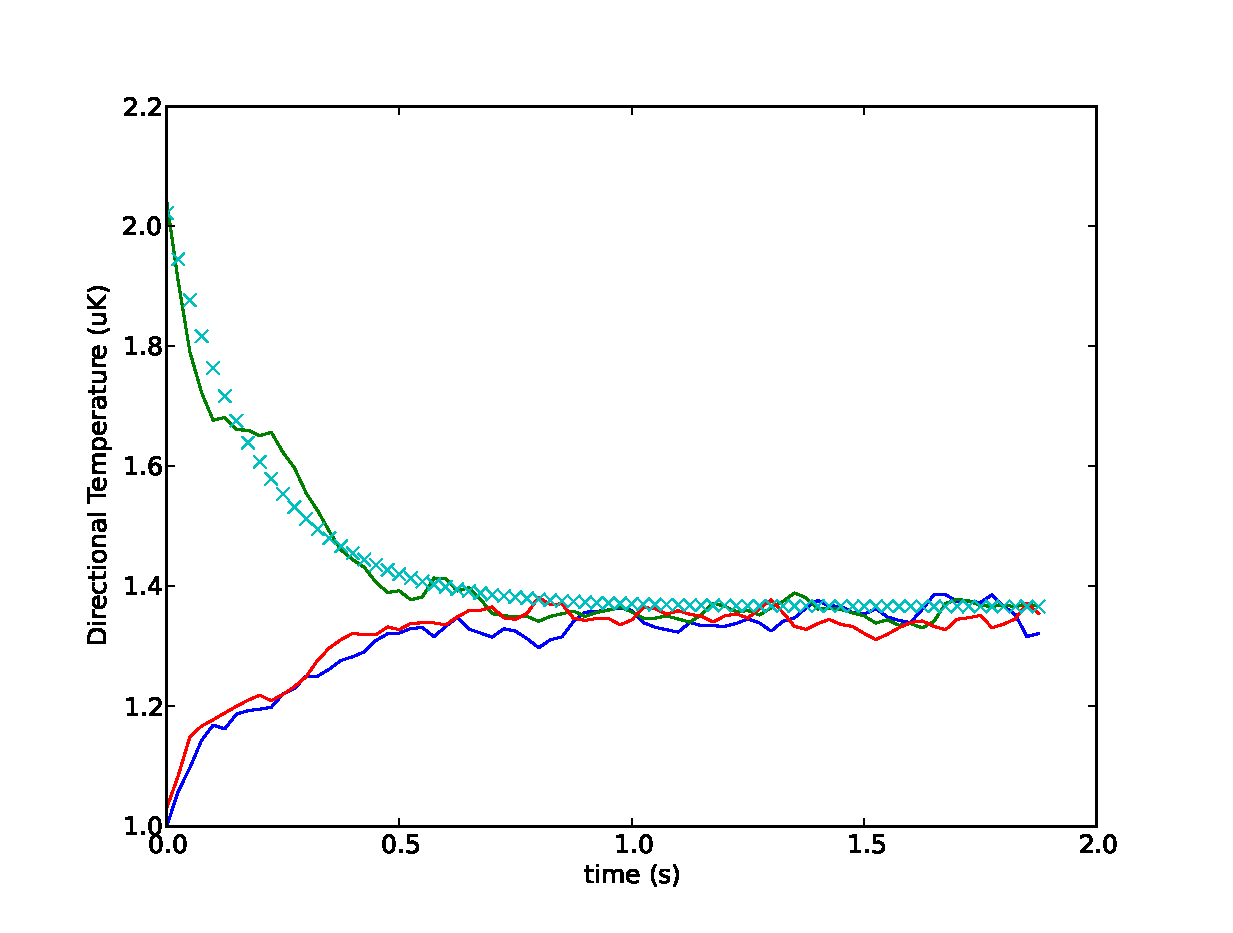
\includegraphics[width=0.525\textwidth]{gfx/Thermalisation/monroeIP}}\quad
\subfloat[Walraven quad gas thermalisation. $\tau_{c}^{-1} / \tau^{-1} = 6.09$]{\label{fig:monroeQ}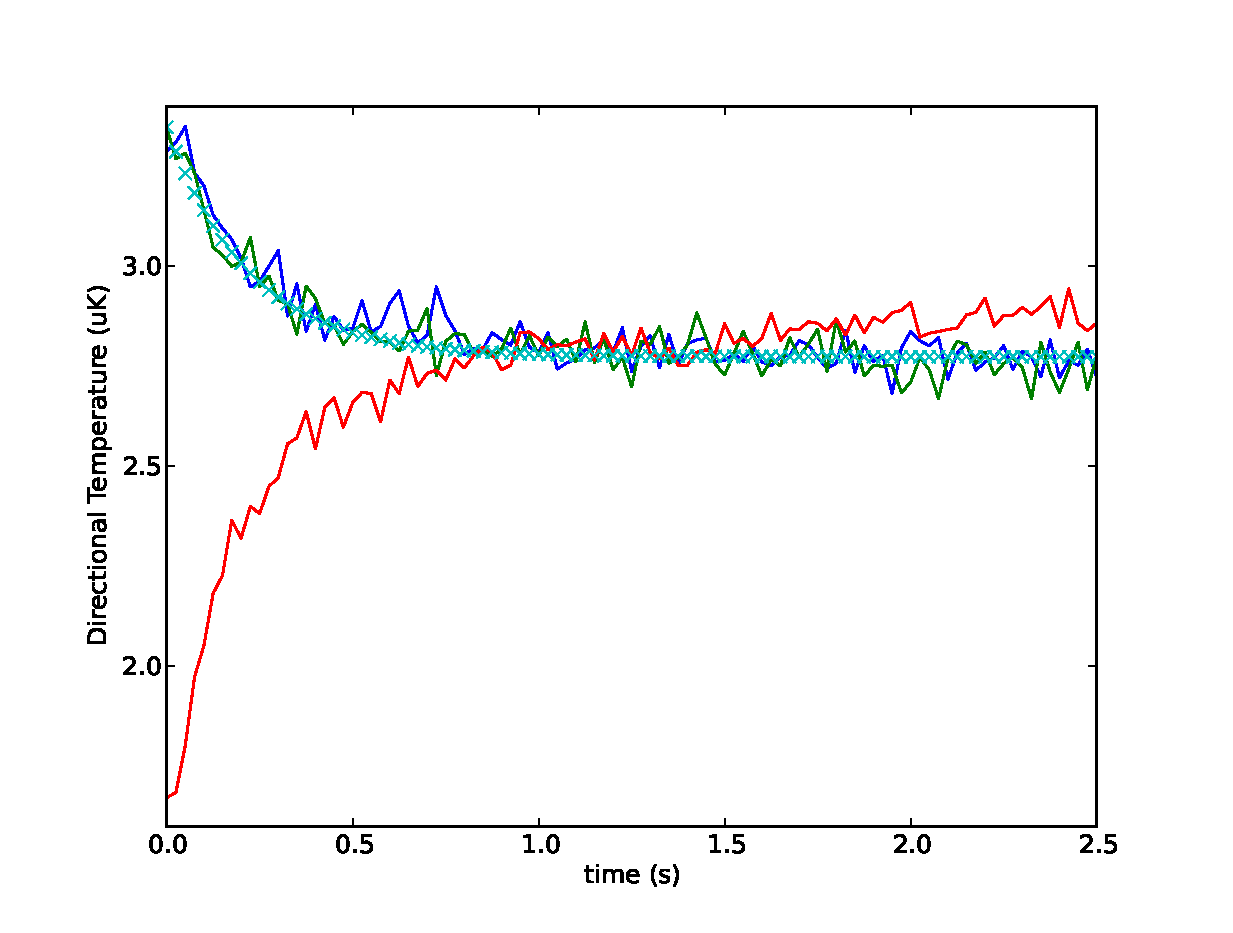
\includegraphics[width=0.525\textwidth]{gfx/Thermalisation/monroeQuad}}%
}
\caption{Walraven rethermalisation. I want to do this simulation for some different perturbation temperatures. One more higher and one lower too.}\label{fig:monroeTherm}
\end{figure}

Also do it for different temperatures or trap numbers.

*** MUST REDO ALL OF THESE SIMULATIONS WITH COLLISIONS WORKING CORRECTLY (I.E. WITH THE NEW SORTING FIX IMPLEMENTED). ***
\marginpar{Comment on directional temperatures being a useful tool for checking that collisions are working effectively. }
%----------------------------------------------------------------------------------------

\section{Evaporation} \label{sec:evaporation}

Compare some results to those predicted by the theory of walraven \cite{Walraven2010} and the other guy \cite{Luiten1996} . 

Say something about the ability to accurately simulate evaporation being important for ensuring the simulation of energy distribution during majorana loss.

As demonstrated by Wu et al \cite{Wu1996, Wu1997} we can use the DSMC method to simulate evaporative cooling.
There has been a lot of theoretical investigation into the evolution of cold gases under forced evaporative cooling \cite{Davis1995, Luiten1996, Holland1996}, giving us a good basis for analysis.
We will use the results of Luiten et al \cite{Luiten1996} to validate to our simulations.
In their work Luiten et al find that the rate of change of total energy due to evaporation is given by 
\begin{equation}    
    \dot{E} = \left( \eta + \frac{W_{\mathrm{ev}}}{V_{\mathrm{ev}}}\right) \dot{N} k_B T, \label{eq:evapEnergy}
\end{equation}
where the effective volume for elastic collisions leading to evaporation, $V_\mathrm{ev}$, is given by
\begin{equation*}
    V_\mathrm{ev} = \frac{\Lambda}{k_B T} \int_0^{\epsilon_t} \rho(\epsilon)\left[\left(\epsilon_t-\epsilon-k_B T\right)e^{-\epsilon/k_B T} + k_B T e^{-\eta}\right]\,d\epsilon
\end{equation*}
and the volume $W_\mathrm{ev} = V_\mathrm{ev} - X_\mathrm{ev} $, with
\begin{equation*}
    X_\mathrm{ev} = \frac{\Lambda}{k_B T} \int_0^{\epsilon_t} \rho(\epsilon)\left[k_B Te^{-\epsilon/k_B T}  - \left(\epsilon_t-\epsilon+k_B T\right)e^{-\eta}\right]\,d\epsilon.
\end{equation*}
If we use the expression for an isotropic power law potential, \autoref{eq:powerlaw} from \autoref{sec:collisionRates}, we can find a (rather complicated) expression for this ratio of volumes
\begin{equation*}
    \frac{X_\mathrm{ev}}{V_\mathrm{ev}} = \frac{2 \left(2 (2 \gamma +2 \eta +5) \eta ^{\gamma +\frac{3}{2}}+e^{\eta } \left((2 \gamma +3) (2 \gamma +5) \Gamma \left(\gamma +\frac{3}{2},\eta \right)-4 \Gamma \left(\gamma +\frac{7}{2}\right)\right)\right)}{e^{\eta } (-2 \gamma +2 \eta -5) \left((2 \gamma +3) (2 \gamma +5) \Gamma \left(\gamma +\frac{3}{2},\eta \right)-4 \Gamma \left(\gamma +\frac{7}{2}\right)\right)-2 (2 \gamma +5)^2 \eta ^{\gamma +\frac{3}{2}}},
\end{equation*}
where $\Gamma\left[a,z\right] = \int_z^\infty t^{a-1}e^{-t}\,dt$ is the incomplete gamma function and $\Gamma\left[a\right] = \int_0^\infty t^{a-1}e^{-t}\,dt$ is the Euler gamma function.
It might not be immediately obvious from the equation above, but for a given $\gamma$ this ratio has a maximum of 1 at $\eta=0$ and is a monotonically decreasing function of $\eta$.
I have included this to illustrate a rather unintuitive result.
That is that the rate of change of the total energy for an evaporatively cooled gas is not only a function of the evaporation parameter $\eta$, but also a function of the trapping parameter $\gamma$.
Perhaps if we reflect on the thermalisation experiments we have done in the previous \autoref{sec:walravenTherm} and \autoref{sec:monroeTherm} it is not so surprising that this is the case.

If we now differentiate the equation for the total energy of the gas, $E=\left(\frac{3}{2} + \gamma\right)Nk_BT$, with respect to time and combine it with \autoref{eq:evapEnergy} we can show
\begin{equation}
    \frac{\dot{T}}{T} = \left(\frac{\eta + \frac{W_\mathrm{ev}}{V_\mathrm{ev}}}{\frac{3}{2}+\gamma}-1\right) \frac{\dot{N}}{N}. \label{eq:tempEvap}
\end{equation}
Keeping in mind the maximal value for $W_\mathrm{ev} / V_\mathrm{ev}$ is 1 we can see from the above that we require $\eta > \gamma + 1/2$ for the temperature to decrease as the number of atoms decreases. 
Further more we can note the larger $\eta$ is the more efficient the evaporative cooling will be \ie a smaller loss of atoms will result in a larger decrease in temperature.

We can also investigate how the density of the gas changes with the number of atoms.
Recall in section \autoref{sec:collisionRates} we claimed the density would \emph{increase} as we \emph{removed} atoms (how can this be?!).
Using the relationship $N=n_0V_e$ and the subsequent derivative $\dot{N} = \dot{n}_0V_e + n_0\dot{V}_e$, and combining this with the results from \autoref{tab:collisionrates} and \autoref{eq:tempEvap} we have
\begin{equation}
    \frac{\dot{n}_0}{n_0} = \left(1-\gamma\left(\frac{\eta + \frac{W_\mathrm{ev}}{V_\mathrm{ev}}}{\frac{3}{2}+\gamma}-1\right)\right) \frac{\dot{N}}{N}. \label{eq:densEvap}
\end{equation}
Thus we see that for the density of the gas to increase as the number of atoms decreases we require that $\eta > \gamma + 3/2 + 3/2\gamma$. 
It is clear from \autoref{eq:densEvap} that the larger $\gamma$ is the greater increase in density we will have for a given loss of atoms.

Finally we can see how the degeneracy parameter, $D=n_0\Lambda^3$, changes with the loss of atoms
\begin{equation}
    \frac{\dot{D}}{D} = \left(\gamma -\eta -\frac{W_\mathrm{ev}}{V_\mathrm{ev}} +\frac{5}{2}\right) \frac{\dot{N}}{N}.
\end{equation}
So for $\eta > \gamma + 3/2$ we will have an increase in the degeneracy parameter as the number of atoms decreases.
Here is the definitive result that drives the desire to evaporate in a quadrupole potential.
We can see that the larger $\gamma$ is the greater the increase in the degeneracy parameter will be for a given $\eta$.
Thus if we can use a quadrupole trap, with $\gamma = 3$, we will reach the quantum limit with the minimum atom loss.

%----------------------------------------------------------------------------------------

\section{DSMC simulations of Evaporation} \label{sec:dsmcevaporation}

Armed with the relationships from \autoref{sec:evaporation} we can investigate the accuracy of the DSMC when applied to the evaporative cooling of cold atoms.

\begin{figure}[bth]
\myfloatalign
\subfloat[$\eta$ should equal 7, here it is equal to 7.86 ]
{\label{fig:dsmchomoerr}
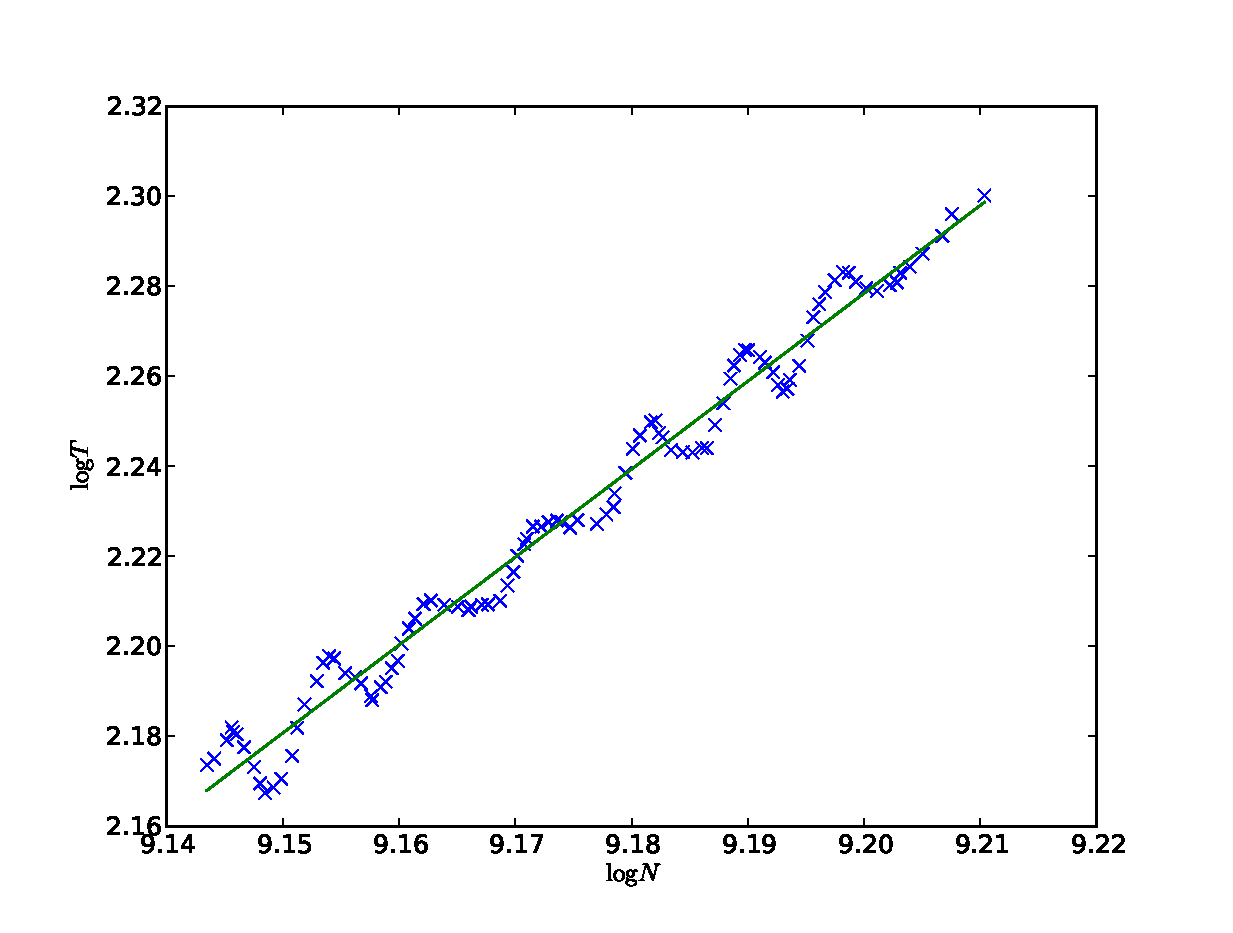
\includegraphics[width=.45\linewidth]{gfx/Evaporation/evapIP}} \quad
\subfloat[I want this to be a plot of n0 vs N.]
{\label{fig:dsmcquaderr}
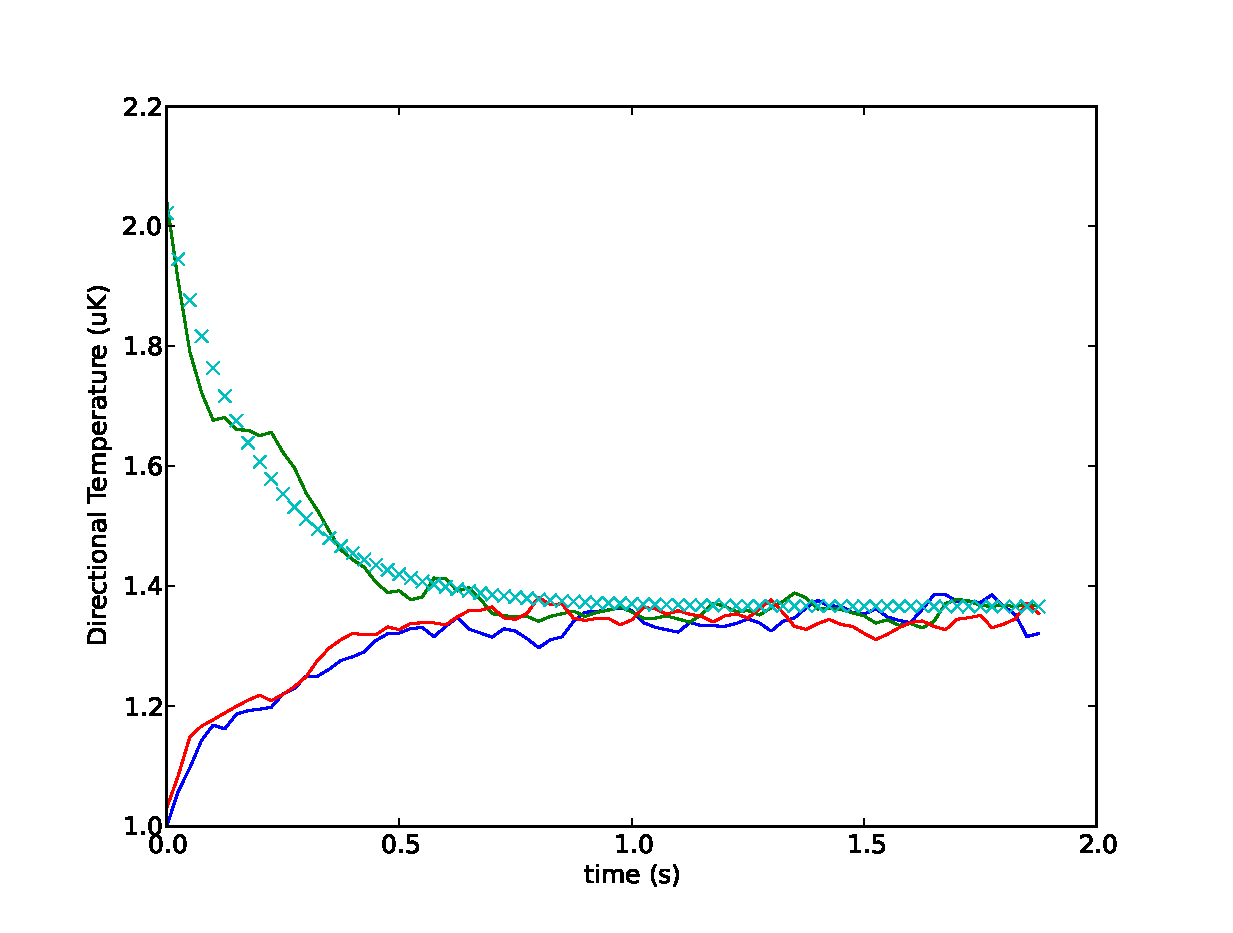
\includegraphics[width=.45\linewidth]{gfx/Thermalisation/monroeIP}}
\subfloat[Not sure what plot tp put here]
{\label{fig:dsmcquaderr}
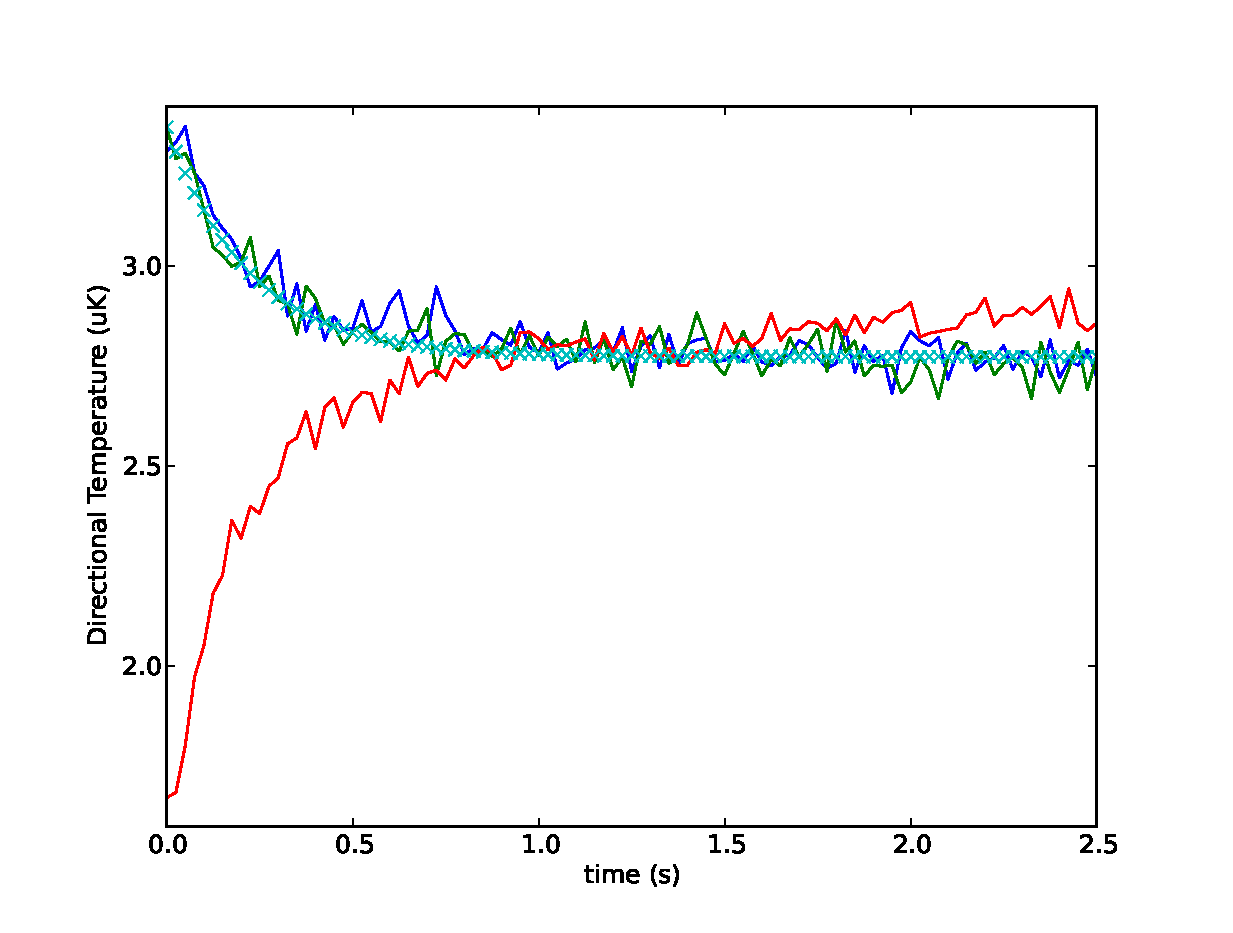
\includegraphics[width=.45\linewidth]{gfx/Thermalisation/monroeQuad}}
\caption[]{IP trap evaporation.}\label{fig:dsmccolerr}
\end{figure}

\begin{figure}[bth]
\myfloatalign
\subfloat[$\eta$ should equal ?(check the paper), here it is equal to 5 ]
{\label{fig:dsmchomoerr}
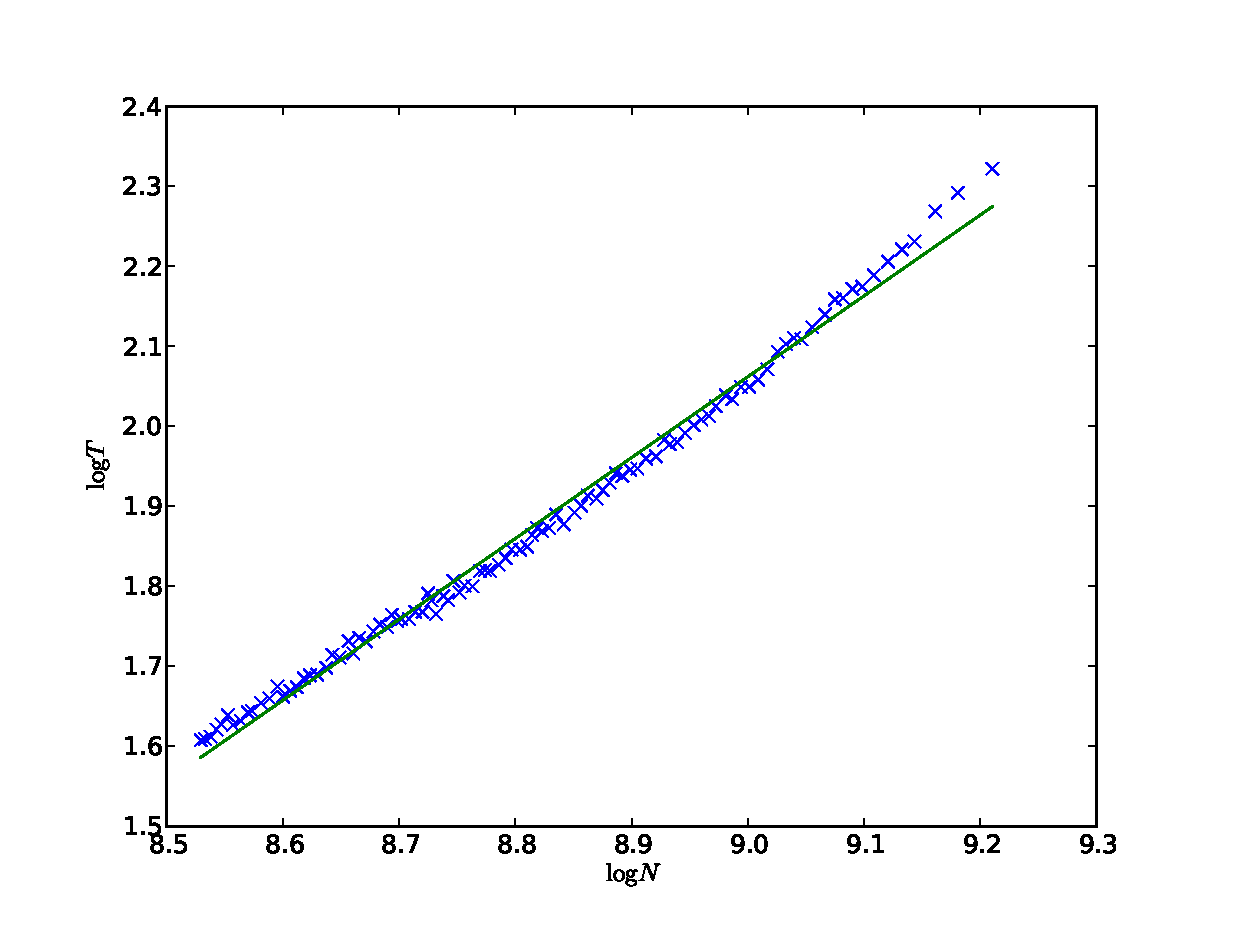
\includegraphics[width=.45\linewidth]{gfx/Evaporation/evapQuad}} \quad
\subfloat[I want this to be a plot of n0 vs N.]
{\label{fig:dsmcquaderr}
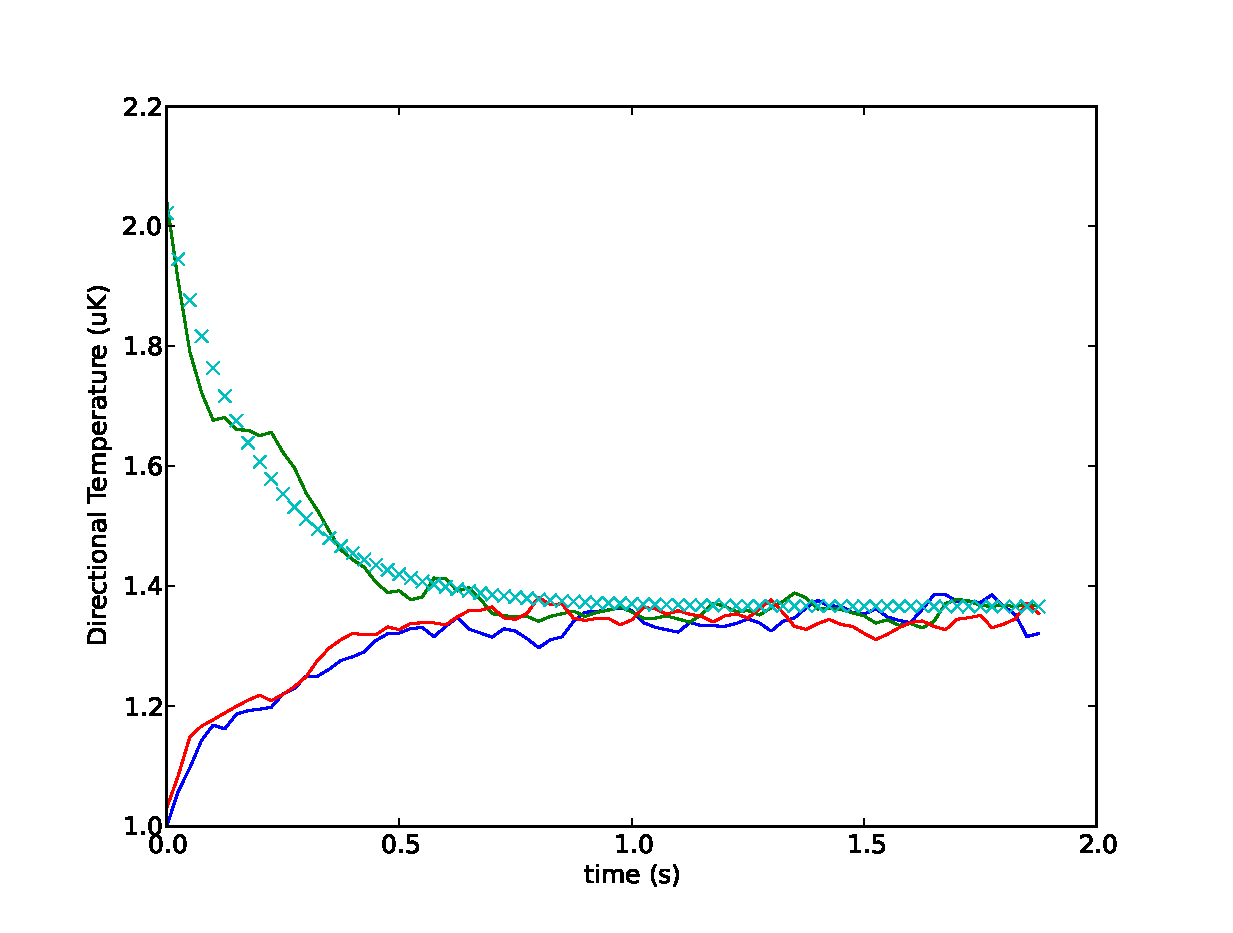
\includegraphics[width=.45\linewidth]{gfx/Thermalisation/monroeIP}}
\subfloat[Not sure what plot tp put here]
{\label{fig:dsmcquaderr}
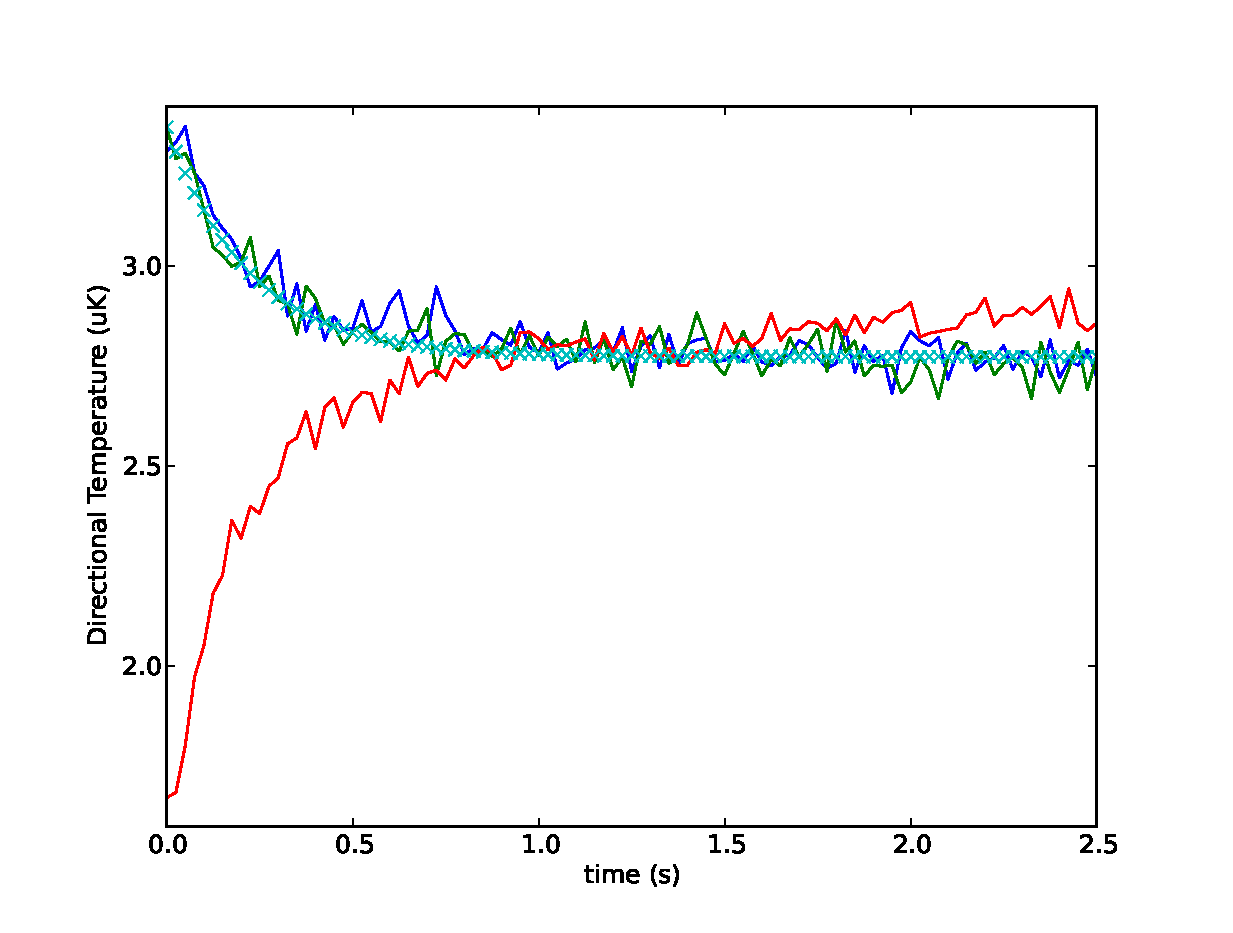
\includegraphics[width=.45\linewidth]{gfx/Thermalisation/monroeQuad}}
\caption[]{Quadrupole trap evaporation.}\label{fig:dsmccolerr}
\end{figure}

\section{Adiabaticity}

Have a look at squeezing the magnetic trap both diabaticaly and adiabatically.